\documentclass[czech,a4paper,22pt]{article}

\setlength{\topmargin}{-3.54cm}
\setlength{\oddsidemargin}{-1cm}
\setlength{\evensidemargin}{-1cm}
\setlength{\textwidth}{17.5cm}
\setlength{\textheight}{25.5cm}

\usepackage[czech]{babel}
\usepackage[utf8]{inputenc}
\usepackage{graphicx}
\usepackage{subfigure}
\usepackage{picins}
\usepackage{amsmath}
\usepackage{color}
\usepackage{latexsym}

\def\modre#1{\textcolor{blue}{#1}}
\def\algn#1{\mbox{\sc #1}}
\def\pp{\hglue 2em}
\def\kw#1{{\bf #1}}
\begin{document}
{\small
\begin{tabular}{p{.6\textwidth}p{.25\textwidth}}

~

\LARGE{\bf A}

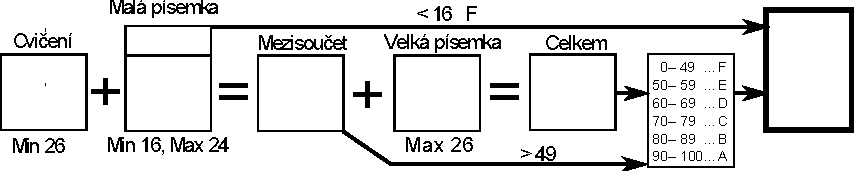
\includegraphics[width=10cm]{hlavicka.pdf}
     &
\begin{tabbing}
  \hspace{1.5cm} \= \hspace{2cm} \= \
   Prijmeni: \> 
ule{3cm}{.1mm}\[.3cm]
   Jmeno:  \> 
ule{3cm}{.1mm}\[.3cm]
   Cvicici:  
   \> $\Box$ Matyas \> $\Box$ Chludil\[.3cm]
   Skupina: 
   \> $\Box$ ct, 12:45 \> $\Box$ st, 12:45 \
   \> $\Box$ ct, 14:30 \> $\Box$ st, 14:30 \ 
   \> $\Box$ ct, 16:15 \> $\Box$ st, 16:15 \
   \> $\Box$ ct, 18:00 \> $\Box$ st, 18:00 \
   
\end{tabbing}
\end{tabular}
}
\begin{enumerate}

                            \large{\item otazka cislo 1 v okruhu 1 \\}
			\hrule
			
                             \begin{description}
                                    \item[a)] odpoved 2 
                                    \item[b)] odpoved 3
                                    \item[c)] odpoved 1
                                    \item[d)] odpoved 4\end{description}
                            
			\hrule
			
                            \large{\item  otazka cislo 1 okruh 2\\}
			\hrule
			
                             \begin{description}
                                    \item[a)] odpoved 2
                                    \item[b)] odpoved 4
                                    \item[c)] odpoved 3
                                    \item[d)] odpoved 1 \end{description}
                            
			\hrule
			\end{enumerate}\newpage
                            \large{\item  otazka cislo 1 okruh 2\\}
			\hrule
			
                             \begin{description}
                                    \item[a)] odpoved 2
                                    \item[b)] odpoved 1 
                                    \item[c)] odpoved 3
                                    \item[d)] odpoved 4\end{description}
                            
			\hrule
			
                            \large{\item otazka cislo 1 v okruhu 1 \\}
			\hrule
			
                             \begin{description}
                                    \item[a)] odpoved 2 
                                    \item[b)] odpoved 1
                                    \item[c)] odpoved 3
                                    \item[d)] odpoved 4\end{description}
                            
			\hrule
			\end{enumerate}\newpage\end{document}